\documentclass{llncs}
\usepackage{tikz}
\usepackage[simplified]{pgf-umlcd}
\usepackage{cite}
\usepackage{listings}
\usepackage{paralist}
%
\begin{document}

\title{LongXact: Making Long-Lived Transactions Easier to Develop}

%% Title
\author{Jo\~{a}o Pedro Carvalho} \institute{T\'{e}cnico de
  Lisboa/Universidade T\'{e}cnica de Lisboa
  \email{joao.pedro.carvalho@ist.utl.pt}}
\maketitle

%% Abstract

\begin{abstract}
  Over the past years, Software Transactional Memories have become
  more and more popular, growing to be something more than simply a
  research topic. On top of that, the concept has been extended to
  encompass persistence, so the concept of Persistent Software
  Transactional Memories was born. In this thesis, I propose an
  extension to PSTM's in order to support the concept of Long-Lived
  Transactions. Some research on the topic has been conducted in the
  field of Database Transactions and Workflow systems. My thesis is
  that supporting Long-Lived Transactions should be done at the
  infrastructural level on Persistent STM's, so this paper will
  describe how those systems can be extended to support Long-Lived
  Transactions.
\end{abstract}

%% Intro

\section{Introduction}

For many years, enterprise applications were developed using
two-tiered architectures. In such architectures, there was typically a
mainframe with great computational power.

Long-Lived Transactions were first described in 1981 as ``[..]
transactions with lifetimes of a few days or
weeks''\cite{gray1981transaction}. At the time, the author said that
the solution for this

-- starts here for now --

In this project, I aim at adding support for Long-Lived Transactions
in applications with Rich Domain Models.  A Rich Domain Model is ``An
object model of the domain that incorporates both behaviour and
data.``, as described by \cite{fowler2003patterns}, meaning that
domain objects hold both their data and the business logic that
manipulates them, as opposed to Anemic Domain Model, in which the
domain objects simply contain data, and the business operations are
handled by a separate Service layer. Also, in a Rich Domain Model,
each domain object typically has an arbitrarily complex web of
associations, multivalued attributes, inheritance, and other Object
Oriented design patterns.

My focus throughout this project will be on applications in which the
Domain Objects are persistent, transactionally updated, and handled
transparently at an infrastructural level (meaning the programmer may
be mostly unaware of the persistence layer).

\section{Long-Lived Transactions}

In this section I provide a concrete example of a Long-Lived
Transaction, aiming to better explain the concept, and to show how
such transactions can be found among many applications. I then show
why it is difficult for a programmer to implement a Long-Lived
Transaction, attempting to motivate why a new approach is needed.

\subsection{What are Long-Lived Transactions?}
\label{sec:what}

As previously described, Long-Lived Transactions are transactions with
a lifetime larger than a typical database transaction. In order to
better understand this concept, consider the following example, found
in the applications of many education institutions.

\begin{figure}
  \centering
  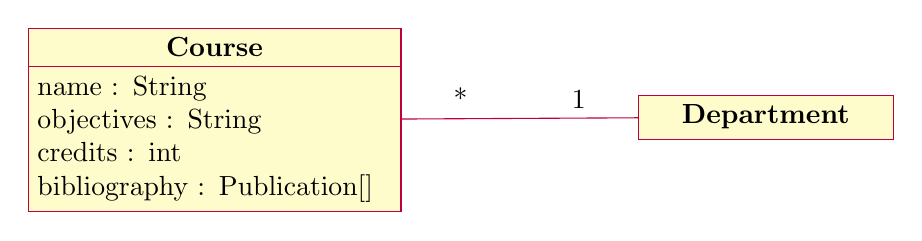
\begin{tikzpicture}

\begin{class}[text width=4.5cm]{Course}{0.5,0}
  \attribute{name : String} \attribute{objectives : String}
  \attribute{credits : int} \attribute{bibliography : Publication[]}
\end{class}

\begin{class}[text width=3cm]{Department}{7.5,-0.85}
\end{class}

\association{Department}{}{1}{Course}{}{*}

\end{tikzpicture}

\caption{Sample Domain Model in UML}
\label{fig:courseDomain}

\end{figure}

In the domain model presented in Figure~\ref{fig:courseDomain}, we
present a simplification of the Course's attributes. A course belongs
to a department, has a name, its objectives, the credits granted upon
completion, and the recommended bibliography. The domain is deemed to
be consistent only if all attributes of Course have a defined value,
and each course must have a department. Each department is responsible
for managing its courses, meaning that it is up to someone who works
in the department to start the process of creating new courses.

Note that the creation of a new course should be executed
transactionally, since it is not desired that other users of the
system are able to see a course in an inconsistent state (either not
connected to any departement and/or without all attributes properly
defined).

The pseudo-code in Listing~\ref{fig:courseCreation} implements the
business operation of creating a new course. Assume that {\bf
  department} is inferred from the user performing the operation.

\lstset{language=Java, basicstyle=\ttfamily, stepnumber=2,
  numbersep=9pt, tabsize=4, frame=single, caption={Pseudo-Code for the
    creation of a new course. A new Course is created, associated with
    its department, and its attributes are filled.},
  label={fig:courseCreation}, captionpos=b}
\begin{lstlisting}
Course course = new Course();
department.addCourse(course);
course.setName(name);
course.setObjectives(objectives);
course.setCredits(credits);
course.setBibliography(bibliography);
\end{lstlisting}

There are several ways to implement this operation. I will now
describe two common scenarios for said implementation.

\subsubsection{Business Transaction in a single interaction}

A possible implementation (most likely, the simplest) of the course
creation operation in a web application is to have a single page in
which the user provides all the required information. Once the
information is submitted, a new Course is created, associated with the
department of the person performing the operation, and all its
attributes are filled according to the information submitted by the
user. The new object is then stored in the database, making it
persistent and available for other users to view.

In this scenario, in which all the information can be provided in a
single user interaction, the transactional guarantees of the operation
are assured by the underlying database (which is assumed to provide
the classic transactional semantics \cite{gray1981transaction}), since
the whole operation can be performed within the scope of a single
database transaction.

An important consequence of implementing the operation in a single
database transaction is that the programmer can manipulate all the
domain objects involved directly. The order in which the modifications
to said objects are performed is irrelevant, as long as the domain is
consistent when the transaction is committed. These are the semantics
typically expected by a programmer of such applications: there may be
instants in which some domain objects are in an inconsistent state
(e.g. before defining the course's bibliography), however this
inconsistent state will never be seen by the other users of the
application. Those users will only see the fully created object once
the operation is committed.

\subsubsection{Business Transaction across multiple interactions}

The model described in the previous scenario, while simple and easy to
implement, may not be suited for every situation. Imagine that instead
of four attributes, Course had 50 attributes. It would then be
unfeasible to ask the user to fill everything out in a single web
page, so the logical solution would be to split the various attributes
in multiple pages, accounting for multiple user interactions.

Let us now assume that the creation of a course is made throughout
three interactions. In the first interaction, the user selects the
course's name, in the second interaction, the user introduces the
objectives and credits, and in the final interaction, the user selects
the bibliography, thus creating the course.

At first glance, it would seem quite easy for a programmer to change
the logic programmed in the first scenario, in order to meet the new
requirements: the programmer would simply have to split the code
performed in a single request into three smaller parts, one to be
executed in each request.

However, having three separate requests implies three different
database transactions, breaking the atomicity and isolation of the
operation. After handling the first request, the persisted domain
would be in an inconsistent state (a course with no attributes but its
name).

The implementation of the business logic must then take this issue
into account, since the programmer cannot write the updates directly
on the domain, requiring manual handling.

This scenario represents what was defined as a Long-Lived Transaction,
in which the Business Operation had a larger lifetime that a single
database transaction (in this particular case, three database
transactions).

\subsection{Why are they difficult to implement?}
\label{sec:difficult}

In this multiple interaction scenario, special care must be taken when
implementing the operation. Like mentioned above, one cannot simple
split the code used in the first scenario.

The programmer has then several choices for the implementation:

\begin{enumerate}
\item Keeping a database transaction open during all the steps of the
  operation.

\item Create a parallel representation of the objects that are being
  manipulated, store them outside the domain, applying the changes
  only in the last interaction.

\item Change the domain model, to represent the consistency state of
  the objects being manipulated. This affects the code that operates
  on that portion of the domain, since it must filter objects that are
  still in an inconsistent state.
\end{enumerate}

It should be clear that any of those solutions is far from trivial to
implement, has some serious consequences, and is an unnecessary burden
to the programmer.

\subsubsection{Keeping a database transaction open}

Given that atomicity and isolation are broken due to the fact that
each interaction with the user is done within its own database
transaction, one could think the solution would be to keep the
database transaction open during the whole business transaction.

However, most modern RDBMs do not cope well with transactions that are
open for arbitrarily large periods of time, since a long lived
database transaction may limit concurrency, cause timeouts and
deadlocks or starve the database's connection pool. All these factors
contribute to making this approach highly undesirable, making the
programmer seek alternative approaches.

\subsubsection{Parallel Representation of the domain}

In this approach, a series of objects similar to the domain objects
are created, and must be managed manually, kept in the user's session
context, outside the domain.

As the complexity of the domain, and the number of objects manipulated
by the operation, grow, the harder it becomes for the programmer to
manually. Ultimately, there is a copy of the whole of the domain
stored in the user's session, waiting for the last transaction to copy
all the information back to the domain transactionally.

This is the opposite of what would be desirable to the programmer, she
should be able to operate directly on the domain.

\subsubsection{Changing the domain model}

Now imagine that an additional requirement is added to the system: the
user may be allowed to log off in the middle of the process, and upon
logging back in, continue the work where she left off. Additionally,
anyone else in the user's department should be able to pick up where
the original user left off. With these requirements, it becomes clear
that simply storing a copy of the domain in session-local storage is
not enough.

Web application containers already provide an application context,
which could potentially solve this issue, however, there are no real
guarantees that the data stored in that context will be kept for an
arbitrarily large period of time (recall that our transaction may span
several days or weeks), meaning that the intermediate data must be
kept persistently, forcing the programmer to be concerned with this
issue.

A possible solution for this requirement is to change our domain
model, by adding a new attribute to the objects being modified (in
this case, Course, as shown in
Figure~\ref{fig:courseDomainState}). The {\bf status} attribute
indicates whether the course is in a consistent state (Published) or
not (Draft). Adding this attribute has a cost, not only the domain is
'polluted' with information that is not relevant to the object being
modeled, but has impact on other functional code across the
application, since course listings must filter out courses that are
still in the Draft status, scattering the filtering code throughout
the application.

\begin{figure}
  \centering
  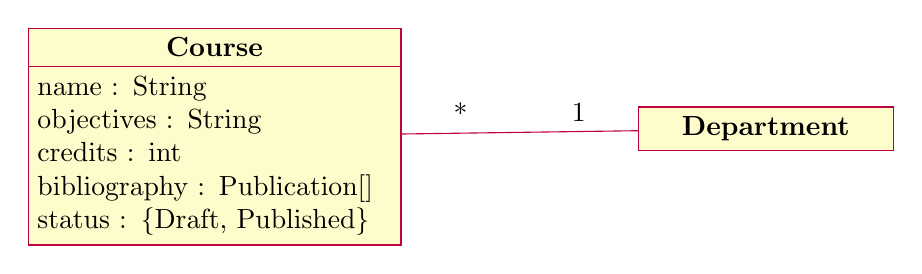
\begin{tikzpicture}

\begin{class}[text width=4.5cm]{Course}{0.5,0}
  \attribute{name : String} \attribute{objectives : String}
  \attribute{credits : int} \attribute{bibliography : Publication[]}
  \attribute{status : \{Draft, Published\}}
\end{class}

\begin{class}[text width=3cm]{Department}{7.5,-1}
\end{class}

\association{Department}{}{1}{Course}{}{*}

\end{tikzpicture}

\caption{Domain Model with state representation}
\label{fig:courseDomainState}

\end{figure}

\subsubsection{Other approaches}

There are other approaches to Long-Lived Transactions, such as using
the Database. There are some DBMSs that announce support for
Long-Lived Transactions, such as Oracle's Workspace Manager. However,
uch support is not standardized, their API's are proprietary,
rendering Web frameworks unusable in those cases (since they generally
support only the SQL standard), forcing the application to be written
against the proprietary API, making it very hard to change and
maintain. All these factors contribute to make this approach
inadmissible for most cases.

\subsection{Applications of LLTs}

Even though the example I just presented was targeted at a system with
a rich domain model, there are several other applications of
Long-Lived Transactions.

\subsubsection{Database Management Systems}

The example provided above is targeted at applications with a rich
domain model, however there are many applications built directly on
top of DBMS's that

\subsubsection{Workflow Systems}

Workflow Management Systems are another area in which Long-Lived
Transactions are interesting. Workflow processes represent business
transactions, consisting in a flow of steps or tasks, each of them
possibly performed by different people.

It is thus vital for Workflow Systems to embrace Long-Lived
Transactions as a core concept, and many approaches have been
developed in this area.

Consider the Course Creation example. Assume that each step of the
operation is executed by a different person. A Workflow Management
System could be a candidate to implement that operation.

\subsection{Objectives}

All this effort makes Long-Lived Transactions a concept that is very
hard to implement, promotes bad software engineering practices
(replication, code scattering, etc), and is difficult to reason
about. My thesis is that the support for Long-Lived Transactions
should be transparent, and at an infrastructural level, relieving the
programmer from this burden.

\section{Related Work}

In this section I describe the various topics in which an attempt to
solve the problem of Long Lived Transactions has been made, namely
Database Management Systems, Workflow Systems and Object Oriented
Transactional Systems.

Also, due to its relevance regarding the solution described in section
4, I briefly present Software Transactional Memories, and how they
cope with short lived transactions.

\subsection{Database world}
\label{sec:rdbms}

\subsubsection{Isolation Levels}
\label{sec:isolation}

In order to better understand the desired isolation level of a
Long-Lived Transaction support system, an analysis of the most common
isolation levels is in order.

Attaining full isolation between transactions, while seemingly
necessary, can oftentimes be a burden to the DBMS, due to the required
overhead. Thus, isolation is, out of the four ACID properties, the one
most often relaxed. Isolation is typically implemented using Locks or
Multiversion concurrency control, which may result in a loss of
concurrency. In order to cope with that fact, several standard
isolation levels have been defined.

In the ANSI/ISO SQL standard\cite{melton1992ansi}, four isolation
levels have been defined (from most to least relaxed):

\begin{itemize}
\item {\bf Read Uncommitted} In this isolation level, read operations
  are performed in a non-locking fashion, thus, {\it Dirty reads} may
  occur. A {\it Dirty read} is defined as a read operation that reads
  data updated by a live (not yet committed) transaction.
\item {\bf Read Committed} In this level, {\it Dirty reads} cannot
  happen, guaranteeing that all reads are {\it Consistent reads}
  (meaning they only read data written by already committed
  transactions). However, multiple reads to the same data location may
  read different values (from transactions that committed in between),
  even within a single transaction.
\item With {\bf Repeatable Read}, all {\it Consistent reads} within
  the same transaction read the snapshot established by the first
  read.
\item {\bf Serializable} is the {\it highest} isolation level defined
  in SQL. Serializability requires repeatable reads, as well as
  guaranteeing that {\it Phantom reads} do not occur. A {\it Phantom
    read} occurs when, in the course of a transaction, two identical
  queries (that act upon a range of values) return a different result
  collection. This can occur when running queries like ``SELECT * FROM
  users WHERE age BETWEEN 10 AND 30;''. If an interleaving transaction
  creates a new user with an age between 10 and 30 years, the second
  run of the query will show a result which contains the new user.
\end{itemize}

In \cite{papadimitriou1979serializability}, an extension to
Serializability is described: Strict Serializability. In addition to
the requirements for Serializability, Strict Serializability requires
that transaction histories are real-time ordered, meaning that all
transactions histories must be ordered in a way consistent with the
precedence order of the operations. In practice, this isolation level
is not implemented by DBMSs, due to its performance impact.

Another common isolation level (not described in SQL-92) is {\bf
  Snapshot Isolation}. In snapshot isolation, all reads made within a
transaction are guaranteed to see a consistent snapshot of the
database, and the transaction itself will only commit if no updates it
has made conflict with any concurrent updates since the
snapshot. Snapshot isolation arose from work on Multiversion
Concurrency Control, and thus did not make it into the lock-based
mindset of the SQL-92 standard.

\subsubsection{Concurrency Control}

*Mention classic books*

*Relaxation of transactional properties*

*Several Papers: \cite{hagmann1991implementing} \cite{garcia1987sagas}
\cite{salem1989altruistic}

\subsubsection{Nested Transactions}

*Mention that the best implementations of LLT's at the database level
provide only Serializability at best*

\subsubsection{Offline Concurrency Patterns}

Martin Fowler, in his book ``Patterns of Enterprise Application
Architecture'' \cite{fowler2003patterns}, introduces a series of
``Offline Concurrency Patters'', as the building blocks for Long-Lived
Transaction support at the application level. In his patterns, Fowler
assumes that a Long-Lived Transaction is run as a series of
short-lived system transactions, whose transactional support is
provided by the underlying DBMS.

The patterns provide a workaround for the fact that the ACID
properties are broken by using several system transactions.

\begin{itemize}
\item {\bf Optimistic Offline Lock} This pattern solves the problem by
  validating that the changes about to be committed by one session (or
  business transaction) don't conflict with the changes of another
  session. This is achieved by, in each system transaction commit,
  validating that the changes about to be committed are consistent,
  making sure that the value previously read by the current session
  was not changed by another session (i.e. obtaining an Optimistic
  Offline Lock).  The most common implementation of this pattern
  consists on associating a version number with the record in the
  system. When a record is loaded, the record's version is kept in the
  session, and that version is used when acquiring the Optimistic
  Offline Lock (by comparing the two versions). Once the lock is
  successfully acquired, the record's version is incremented, and the
  system transaction can be committed. If the lock cannot be acquired,
  a conflict is detected, the current system transaction is rolled
  back, and the business transaction must either abort or attempt to
  resolve the conflict and retry.

\item {\bf Pessimistic Offline Lock} This patterns prevents conflicts
  by avoiding them all together. It forces a business transaction to
  acquire a lock in each record before using it, so once you begin the
  business transaction, you are mostly sure that it will complete
  without concurrency control issues. These locks however, are not
  database-level locks, but are instead high-level, typically managed
  by a lock manager in the application, and can have various
  granularities (which will have different impacts on system
  performance). In this pattern, whenever a business transaction
  wishes to access a record (for either read or write), it must
  acquire a lock with the lock manager, assuring that a business
  transaction that wishes to write for that particular record is the
  only one doing so.
\end{itemize}

Typically {\bf Optimistic Offline Lock}s are used in an environment
where conflicts are expected to be low. If conflicts are likely, it is
not good user experience to report a conflict after the user finished
his work and is ready to commit. In that case, a {\bf Pessimistic
  Offline Lock} is in order, avoiding throwing away work, since
conflicts can be detected early in the transaction. Also, if the cost
of a conflict is too high, no matter its likelihood, this is the
appropriate pattern.

Although with the use of these patterns, the development of Long-Lived
Transactions is facilitated, they still require reasoning from the
programmer.

\subsection{Workflow Management Systems}

A Workflow Process is described as a sequence of connected steps (or
activities), with special emphasis on the on the flow paradigm, where
each step of the process follows the precedent with no gap, and ends
just before the next step can begin. A Workflow Process typically has
a long duration, involves many users (in fact, each step is typically
executed by a different users), and ranges across a variety of
heterogeneous systems. Individual activities range from computer
programs and applications to human activities such as meetings and
decision making.

Workflow Management Systems (WFMSs) are computer systems that manage
user-defined Workflow processes for different types of jobs and
processes. WMSs assign to each step the person/group responsible for
that step, and once the step is finished, notify the responsible for
the next step, as well as making sure they get the data they need for
that step, as well as the subsequent steps.

In such systems, it is common to provide transactional guarantees to
the process execution. Note that in this context, there is a clear
separation between {\it Business Transaction} and {\it System
  Transaction}. In this case, the {\it Business Transaction} is the
process as a whole, which may be executed via several {\it System
  Transactions}.

However, there is one major difference between typical transaction
systems and WFMSs, since in the later the system has no way of
controlling the application between successive invocation of the
process's activities.

In this document I will use an abstract model to describe Workflow
Processes, using the following concepts:
\begin{itemize}
\item {\bf Process} is a description of the sequence of steps
  necessary to achieve a goal. A process consists of activities and
  data.
\item {\bf Activity} is each step within a process. Activities have a
  name, pre and post-conditions, and a series of constraints.
\item {\bf Control Flow} is the order in which activities are
  executed.
\item {\bf Data Flow} is the mapping between the inputs/outputs of the
  data required by the activities.
\item {\bf Conditions} specify the circumstances in which certain
  events will happen. {\it Transition Conditions} specify whether a
  certain activity may or may not start. {\it Start Conditions}
  specify when an activity is actually started, either by all its
  triggering events (AND) or by just one (OR). {\it Exit Conditions}
  specify whether an activity has finished successfully.
\end{itemize}
In this model, an activity with no incoming activities is considered a
{\it Start Activity}. A process is considered finished once all its
activities are terminated.

Over the years, many Workflow Modelling Languages have been devised,
and in fact, it is still a very active area of research. Examples of
such languages are YAWL \cite{van2005yawl}, AWGL
\cite{fahringer2005specification}, UEML \cite{vernadat2002ueml} among
many others.

One of the biggest challenges with WFMS is that due to its disparity
from the transaction models provided by the ``regular'' transaction
support systems, such as Long-Lived Transaction support. Regarding
correctness and reliability, we are facing major differences, since
WFMSs provide no significant support for recovery and failure
handling, leaving the user with the task of determining the actions
necessary to recover consistency issues and determining which
activities are needed to recover from an exception, while
transactional systems embrace recovery as a core concept.

In most WFMSs the execution of a process is persistent, in the sense
that in case of a failure, the process will stop, until the failures
have been fixed, and then resumed. In case the system fails while an
activity is executing, the system is not notified, and the work
performed by that activity must be manually reverted.

I will now look into several approaches devised to add transactional
support to WFMSs, in which support for Long-Lived Transactions is a
prominent concern.

\subsubsection{Sagas}

Garcia-Molina and K. Salem proposed, in their 1987 paper, the notion
of sagas \cite{garcia1987sagas}. The basic idea of the saga model is
to allow a transaction to release resources prior to committing. A
Long-Lived Transaction is a saga, if it can be seen as a sequence of
sub-transactions that can be interleaved in any way with other
transactions. Each sub-transaction in the sage guarantees that the
ACID properties on the database are preserved.

Partial executions of the saga are undesirable, so the DBMS is
responsible for guaranteeing that either all transactions in a saga
are successfully completed, or compensation actions are run to amend
the partial execution. Thus, each sub-transaction is associated with a
compensating transaction, which undoes the changes performed by the
original transaction. Note that this action does not necessarily
return the database to its original state, but instead acts upon the
``business state'' of the application.

More formally, consider a saga $T$, consisting of sub-transactions
$T_1, T_2, \ldots, T_n$, and compensating actions $CT_1, CT_2, \ldots,
CT_n$. The system guarantees that either the sequence $T_1, T_2,
\ldots, T_n$ is executed (meaning the whole saga is executed), or
$T_1, T_2, \ldots, T_j,CT_j, \ldots, CT_2, CT_1$ for some $0 \le j \le
n$, will be executed (meaning that a failure occurred at $T_{j+1}$,
causing the previously executed sub-transactions to be compensated).

Due to its nature, it is straightforward to translated a saga into a
workflow process. Each activity in the process is modeled as a
sub-transaction, and has an associated compensating transaction. Each
activity has an incoming condition which evaluates to true when the
previous sub-transaction is successfully committed (meaning that the
previous activity was concluded), meaning that execution of the
process can proceed.

If one of the sub-transactions aborts, the corresponding outgoing
condition is evaluated to false, and no other activity in that path
will be executed, making the process evolve in the path of the
compensating activities.

\subsubsection{Why are these systems unfit}

\cite{798492}

*Exception Handling systems*

*Explain why those solutions are not good, since they *may* break ACI
of the ACID model*

\subsection{Object/Relational Mapping}

Due to the increase in popularity of object-oriented programming, a
large number of Object/Relational Mapping (ORM) tools have arisen over
the past few years\cite{orm}. These tools range from simple data
access layer abstractions (which simply abstract the necessary
instructions to perform the desired operation), to fully fledged
tools, which handle every aspect of the Object/Relational Mapping,
making the underlying database completely transparent to the
programmer.

Object/Relational Mapping tools are available for a great number of
languages. For Java, there are two competing persistence standars:
Java Persistence API (JPA) and Java Data Objects (JDO). Both
specifications allow a programmer to create domain entities by
decorating Plain Old Java Objects (POJOs) with annotations, making the
persistence layer transparent to the programmer. While JDO provides a
larger number of features then JPA, the later has seen greater
adoption by the community, both in terms of usage and support.

The most well-known implementations of the JPA are Hibernate,
DataNucleus, OpenJPA and EclipseLink. Other ORM tools include
DatabaseObjects (.NET), NHibernate (Hibernate for .NET), CoreData
(Objective-C), CodeIgniter (PHP) and Django (Python).

In order to provide transactional support for domain objects, ORM's
typically use delegate transaction management to the underlying
Database (which is assumed to provide full ACID support). In fact, as
of this writing, all the examples shown above operate this way. Thus,
Long-Lived Transaction support in ORM tools is largely dependent on
the underlying DBMS, presenting the same challenges as described in
\ref{sec:rdbms}.

Given the popularity of Java, I will now focus on the JPA, and one of
its most popular implementations, Hibernate, in order to understand
how they cope with Long Lived Transactions. Note that despite the
concreteness of the examples presented, their concepts are generic
enough to be applied to any other ORM tool.

\subsubsection{JPA Optimistic Concurrency Control}

The specification of the Java Persistence API assumes the use of
optimistic concurrency control (or optimistic locking). In this
context, optimistic locking is used to prevent the database from
holding on to critical resources, potentially causing high degrees of
contention.  This is achieved by operating directly on the domain
objects, potentially delaying the propagation of the changes made to
the objects.

As part of the JPA, there is the concept of Version field. This field
allows ``disconnected operation'', meaning that the reads/writes from
the database are deferred until a checkpoint or the end of
transaction. When using this optimistic approach, all the versions of
the objects used in the transaction are checked against the version
present in the database, thus ensuring that no dirty reads will occur.

\subsubsection{Hibernate Long Conversations}

Hibernate supports the concept of ``Long Conversations'' by allowing a
session\footnote{A Hibernate session implements the Unit of Work
  design pattern \cite{fowler2003patterns}.} to remain open as long as
the user interaction lasts, potentially executing multiple database
transactions. However, the programmer is responsible for ensuring the
atomicity and isolation of the business transaction, by following a
very strict pattern: all transactions but the last must only read
data, only the last database transaction can update data. Hibernate
assists the programmer in verifying that the data read across the
multiple transactions is consistent, using an object versioning
mechanism. However, this verification only works if all the data
required for the application is read within the first database
transaction.

This support is not good enough for several reasons:

\begin{itemize}
\item It imposes a pattern that may not be suited for many
  applications.
\item All the state of the transaction is kept in memory, which may
  cause the application to run out of memory in very large
  transactions.
\item The session is not kept persistent. If the application server
  restarts in the middle of the transaction, all data is lost.
\item Despite the versioning support, this system only supports the
  ``Repeatable Read'' isolation level (see
  \ref{sec:isolation}). Suppose that a database transaction other than
  the first (T2) reads an object, which was committed concurrently (by
  T3) between the first transaction and T2. T2 will read the value
  written by T3, and the Long Transaction is not serializable.
\end{itemize}

All of this reasons violate the desired properties described in
\ref{sec:difficult}, making this system undesirable.

\subsection{Software Transactional Memories}
\label{sec:stm}

Given that the solution I propose in Section \ref{sec:arch} is built
upon a Software Transactional Memory (STM), a brief introduction to
the topic is in order.

The original idea behing Transactional Memories (TM) is to provide
efficient lock-free data structures for highly concurrent systems
\cite{herlihy1993transactional} using hardware. Its main goal is to
free programmers from using locks and monitors to manage concurrent
accesses to shared data. Managing lock granularity and composability
is a cumbersome and error-prone task, and may lead to unwanted
situations such as deadlocks. Over the years, the original concept of
Hardware Transactional Memories has evolved, giving birth to Software
Transactional Memories. 

Software Transactional Memories bring into the realm of programming
languages, the age-old notion of transactions, well-known in the area
of DBMSs. However, unlike those, STMs are not concerned with the
Durability property of the ACID model, and thus, many STM
implementations have little in common with their database
counterparts. 

There have been several recent proposals for STM implementations, such
as those described in \cite{cachopo2006versioned},
\cite{herlihy2003software}, \cite{marathe2005adaptive},
\cite{dice2006transactional}, \cite{riegel2006lazy} and 
\cite{marathe2006lowering}.

STMs use transactions to isolate memory operations in atomic Units of
Work. A transaction typically contains a Read Set and Write Set, used
to register its read and write operations, respectively. The STM
provides a series of mutable memory locations that can be read from or
written to. It is up to the programmer to confine all of the
application's mutable state to these memory locations, while it is the
responsibility of the STM to guarantee that concurrent accesses to
such memory locations are correct according to the specified
correctness criteria.

\subsubsection{Correctness Criteria}

In Section~\ref{sec:isolation}, I presented the typical isolation
levels (or correctness criteria) that can be found in DBMS. In
\cite{guerraoui2008correctness}, the author claims that the
``traditional'' correctness criteria are unfit for TM implementations,
and proposes the {\it opacity} criterion. Opacity is described as a
safety property that assures that ``[...] (1) all operations performed
by every {\it committed} transaction appear as if they happened at
some single, indivisible point during the transaction lifetime, (2) no
operation performed by any {\it aborted} transaction is ever visible
to other transactions (including live ones), and (3) every transaction
always observes a {\it consistent} state of the system.'', meaning
that unlike Serializability, even {\it non-committed} transactions are
prevented from accessing inconsistent states. This correctness
criteria is ensured by most TM systems.

\subsection{Persistent STMs}

Over the years, Enterprise Application architecture has evolved at a
very fast pace. However, one aspect has remained constant: they still
rely on a relational database to handle both data persistence and
transactional support. In \cite{fernandes2011strict}, the authors
argue that such design, while once justified by hardware limitations,
is no longer suited for today modern applications.

A new architecture was proposed, using a Software Transactional Memory
for transaction support at the application server tier, shifting the
responsibility from the DBMS to the application server. The database
still plays an important role in this architecture, due to the fact
that the STM must be extended to support persistence (PSTMs).

By shifting the responsibility for transaction handling to the STM,
enterprise applications can benefit from the many advancements in the
STM area, such as multi-core machine scaling, stronger correctness
guarantees and nonblocking progress conditions such as lock freedom
\cite{fernandes2011lock}.

Using a PSTM, enterprise application developers no longer have to
trade correctness for performance. Modern PSTM implementations allow
for Strict Serializability, while providing better performance than
regular DBMSs, yielding a throughput increase of up to 23 times
\cite{fernandes2011strict}. 

Another advantage of PSTMs is that, like in STMs, the programmer
benefits from a much simpler and transparent programming model,
allowing for much cleaner and maintainable code, better composability
by using lock-free data structures, making the process of translating
business requirements to code much simpler and bug-free.

In this project, I aim at extending the PSTM model, by adding the
necessary building blocks to support Long-Lived Transactions
(described in Section~\ref{sec:arch}).

\section{Solution Architecture}
\label{sec:arch}

In this section I will describe the architecture of my proposed
solution, as well as a small introduction to the Fenix Framework
\cite{fernandes2011strict}, in which it will be implemented.

\subsection{Transactional Contexts}

The main goal of this solution is to relieve programmers of the burden
of dealing with Long-Lived Transactions, making the effort needed to
program one similar to the effort of programming a regular
transaction. So, what does the single interaction scenario has that
makes it so easy to program? It has a single transactional context
that spans the whole operation (provided by the database transaction,
given that they have the same lifespan). In the second scenario the
database transaction was shorter than the whole operation, so the
context was lost in each step.

The main concept of the proposed architecture is then the {\bf
  Transactional Context}. It is represented as a first-class domain
entity in our rich domain model, making it persistent (unlike the
context provided by a single database transaction) and
transactional. With this persistent context, the programmer no longer
needs to rely on the database to provide the transactional semantics
of the operation.

\begin{figure}
  \centering
  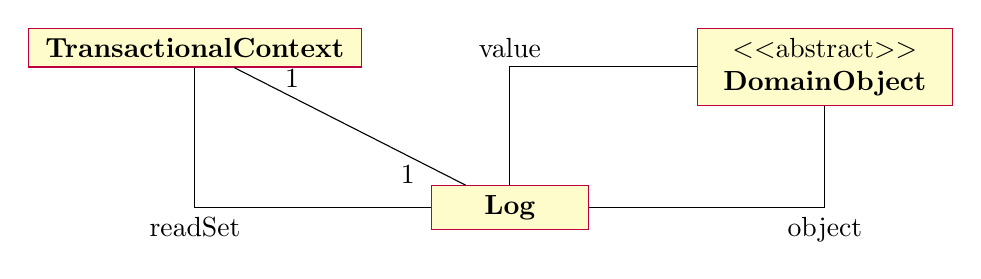
\begin{tikzpicture}

    \begin{class}[text width=4cm]{TransactionalContext}{0,0}
    \end{class}

    \begin{class}[text width=1.2cm,minimum height=5em]{Log}{4,-2}
    \end{class}

    \begin{abstractclass}[text width=3cm]{DomainObject}{8,0}
    \end{abstractclass}

    \draw[umlcd style school] (DomainObject) |-node[below, sloped,
    black]{object} (Log);

    \draw[umlcd style school] (DomainObject) -| node[above, black]
    {value} (Log);

    \draw[umlcd style school] (TransactionalContext) |- node[below,
    black] {readSet} (Log);

    \draw[umlcd style school] (TransactionalContext) -- node[near
    start, above, black]{1} (Log) node[near end, below, black]{1};
  \end{tikzpicture}

  \caption{Transactional Context}
  \label{fig:transactionalContext}

\end{figure}

Figure~\ref{fig:transactionalContext} presents the conceptual model of
the Transactional Context. Since it is a first-class entity, it can be
manipulated just like any other domain object. Its purpose is to keep
all the changes made to the domain objects during the transaction,
keeping those changes isolated from code executing outside this
context.

The Transactional Context has two sets of {\bf Log}s representing both
the read set and the write set of the transaction. A Log contains a
reference to the original object it refers to, and a
Transactional-Local copy of the value of the object. In case of a Log
for a read operation, the value is a snapshot of the object when it
was first read. In the Log for a write operation, the log will retain
the value being written.

Any read operation will read the value stored in the Log for that
particular object (whether it has been modified outside the context or
not), or create a new Log entry if it's the first time the object is
being accessed. A write operation will behave similarly, writing the
new value to the corresponding Log entry. It is important to note that
there is at most one Log entry per object.

Collaboration from the methods that get/set values of the domain
objects is required, since those methods must be aware of the presence
of the transactional context. Depending on whether the method performs
a read or write operation, it must access the corresponding Log of the
current context in order to read/modify the snapshot/copy of the
object's attributes.

Transactional contexts can be either aborted or committed. Aborting a
transactional context simply discards all associated Log entries,
while committing atomically merges the Write Set with the domain. This
operation must obey to the same consistency rules as any regular
transaction, all objects in both Sets must be in a consistent state
with the objects outside the context.

\subsection{Fenix Framework}

STMs, PSTMs, DML

\ref{sec:stm}

\cite{cachopo2006versioned}

Describe that the solution will be build on top of the Fenix Framework
core, plus JVSTM, making it agnostic to the specific persistence
backend in use.

\subsection{Programming Model}

I previously presented the concept of Transactional Context as the
basic building block for Long-Lived Transactions. However, useful as
they may be, Transactional Contexts are not business operations.

The main idea is that every business operation that has transactional
requirements should execute within a transactional context. But due to
the fact that the operation may have several steps, one must keep
track of Transactional Context, so it is used in all steps of the
operation.

Since manually keeping track of the context can be cumbersome, and
should be done transparently, a new concept is introduced: {\bf
  Transactional Business Operation} (TBO). As shown in
Figure~\ref{fig:TBO}, a TBO not only is a first-class entity that
represents a particular business operation, but also holds its
transactional context. The TBO is then responsible for
\begin{inparaenum}[\itshape 1\upshape)]
\item Managing the life-cycle of the Transactional Context
\item Ensuring that the several steps of the operation execute within
  the operation's context.
\end{inparaenum}

\begin{figure}
  \centering
  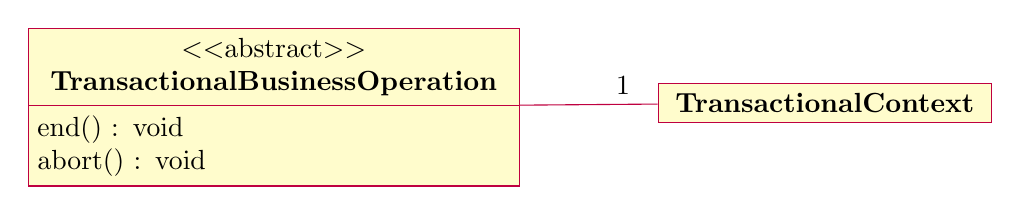
\begin{tikzpicture}

\begin{abstractclass}[text width=6cm]{TransactionalBusinessOperation}{0,0}
  \operation{end() : void} \operation{abort() : void}
\end{abstractclass}

\begin{class}[text width=4cm]{TransactionalContext}{7,-0.7}
\end{class}

\association{TransactionalBusinessOperation}{}{}{TransactionalContext}{1}{}

\end{tikzpicture}

\caption{Transactional Business Operation}
\label{fig:TBO}

\end{figure}

\subsubsection{Instantiating a new TBO}

Instantiating a TBO will also instantiate its associated transactional
context. In order for a method to execute within the context
associated to the TBO, the programmer must simply annotate the method
with the @Step annotation. This will assure that any invocations of
the method will execute within the context of that
operation. Listing~\ref{lst:tcMethod} shows the pseudo-code that will
be injected in the methods to assure this property. The methods
getCurrentTC() and setCurrentTC() allow access and modification of the
current transactional context, which may be stored in a thread-local
variable.

\lstset{language=Java, frame=single, caption={Code to ensure each step
    runs within the operation's transactional context},
  label={lst:tcMethod}}
\begin{lstlisting}
TransactionalContext savedContext = getCurrentTC();
try {
  setCurrentTC(this.getContext());
  // invoke step i of this operation
  if(isLast) {
    end();
  }
} finally {
  setCurrentTC(savedContext);
}
\end{lstlisting}

\subsubsection{Getting the reference to a TBO}

Given that the TBO is modelled as a first class domain entity, it can
be directly associated with its logical owner (e.g. the user who
created it, the department it belongs to, etc).

Getting a reference to the TBO between its various steps (recall that
the application may be restarted, losing all session data) may be as
simple as asking the user to select a pending operation from the list
of operations associated to that user. The framework is flexible
enough to allow for a great number of ways to implement this step.

\subsubsection{Ending the Operation}

There are three ways for a TBO to finish:
\begin{enumerate}
\item By invoking the abort() method of the TBO, which will explicitly
  discard the modifications performed in the context of this
  operation, delete the transactional context, and lastly, the TBO
  itself.

\item By invoking the end() method of the TBO, which will attempt to
  commit the modifications performed by the operation. In case the
  operation cannot be committed, an exception is thrown. If the commit
  is successful, both the TBO and its context are deleted.

\item By invoking a method annotated with @Step, with the {\it last}
  parameter set to {\it true}. This method allows the programmer to
  define a last step, which will automatically commit the operation
  once invoked. The semantics of committing in this case is similar to
  the one provided by calling end(). This is the preferable way of
  ending a TBO, in my opinion, it is the most natural to the
  programmer.
\end{enumerate}

\subsection{Revisiting the Example}

In this section I briefly present a modelling of the example
introduced in section~\ref{sec:what}, using the proposed architecture.

The architecture includes the concept of TBO, so a {\bf
  CourseCreationOperation} is created. This class extends {\bf
  TransactionalBusinessOperation}, and is associated with the course
being created (which is only visible within the context of the
operation until it commits) and the department for which the course is
being created.

An implementation of the {\bf CourseCreationOperation} class is
presented in Listing~\ref{lst:courseTBO}. Each step of the user
interaction is implemented in a single method, annotated with
@Step. Since defining the bibliography is the last step of the
operation, the 'setBibliography()' is annotated with 'last = true',
meaning that after its invocation, the operation will attempt to
commit, making the new course visible to every other user in the
system.

\lstset{language=Java,frame=single,caption={Code for the
    CourseCreationOperation class}, label={lst:courseTBO}}
\begin{lstlisting}
public class CourseCreationOperation 
       extends TransactionalBusinessOperation {    

  @Step
  public void makeNewCourse(Department department,
                            String courseName) {
    this.setDepartment(department);
    this.setNewCourse(new Course(department));
    this.getNewCourse().setCourseName(courseName);
  }

  @Step
  public void setObjectives(String objectives,
                            int credits) {
    this.getNewCourse().setObjectives(objectives);
    this.getNewCourse().setCredits(credits);
  }

  @Step(last = true)
  public void setBibliography
              (Publication[] bibliography) {
    this.getNewCourse().setBibliography(bibliography);
  }
}
\end{lstlisting}

\subsection{Conflict Handling}

Conflict reduction is a topic for which much research has been done
over the past few years.

\section{Evaluation}

The final evaluation of this project will be measured in terms of: -
Programmer effort needed to use LLT's - Performance, throughput,
Commit/Abort ratios, interleaving LLTs with 'regular' transactions

\section{Conclusion}

\subsection{Schedule}

\bibliography{thesis.bib} \bibliographystyle{plain}
\end{document}
